\documentclass[ngerman,12pt]{scrartcl}
% TODO: Was ist eine API / REST-API
% Setup {{{1
% Packages {{{2
\usepackage[backend=biber]{biblatex}
\usepackage[margin=1in]{geometry}
\usepackage{amsfonts, amsmath, amssymb}
\usepackage{babel}
\usepackage{graphicx}
\usepackage{float}
\usepackage[utf8]{inputenc}
\usepackage{fancyhdr}
\usepackage{tikz}
\usepackage{csquotes}
\usepackage[gen]{eurosym}
\usepackage{mathptmx}
\usepackage[scaled=0.9]{helvet}
\usepackage{courier}
\usepackage[T1]{fontenc}
\usepackage{hyperref}
\usepackage{wrapfig}

% Heading {{{2
\pagestyle{fancy}
\fancyhead{}
\fancyfoot{}
\fancyhead[L]{\slshape \MakeUppercase{Informatik Jahresarbeit}\/}
\fancyhead[R]{\slshape Jasper Levin Spahl\/}
\fancyhead[C]{\thepage}
%\renewcommand{\headrulewidth}{0pt}

% Paragraph {{{2
%\parindent 0ex
\setlength{\parindent}{1em}
\setlength{\parskip}{1em}
\renewcommand{\baselinestretch}{1.1}
% }}}
\author{Jasper Levin Spahl}
% Tikz Setup {{{2
\usetikzlibrary{shapes.geometric, arrows.meta}
% Bibliograthy Setup {{{2
\addbibresource{quellen.bib}

\begin{document}
% Titlepage {{{2
\begin{titlepage}
\begin{center}
\vspace*{1cm}

\Large{\textbf{Informatik}}\\
\Large{\textbf{Jahresarbeit}}\\
\vfill
\line(1,0){400}\\[1mm]
\huge{\textbf{Der Smarte Bienenstock}}\\[3mm]
\Large{\textbf{- 12 Kss -}}\\
\line(1,0){400}\\
\vfill
Jasper Levin Spahl\\
Klasse: 12Kss\\
\today\\
\end{center}
\end{titlepage}

% Table of contents {{{2
\tableofcontents
\thispagestyle{empty}
\clearpage
\setcounter{page}{1}

% Einleitung {{{1
\section{Einleitung}

Bei der Auswahl des Themas meiner Jahresarbeit war ich lang unentschlossen.
Ich wusste sofort, dass ich entweder etwas kreatives oder etwas Im It-Bereich machen wollte.
Meine erste Idee war es einen Lichtwecker zubauen.
Ich bemerkte jedoch als ich damit fast fertig war das, dass ganze sehr viel leichter umzusetzen war, sodass ich damit keine komplette Jahresarbeit füllen konnte.
Mir gefiel allerdings das Thema Smarthome/Homeautomation.
Letztendlich brachte mich mein Vater auf die Idee.
Er erzählte mir vom einem Freunde der eine Bienenstockwaage besitzt.
Mit hilft so einer Bienenstockwaage kann man überwachen wie viel Honig sich gerade in dem Stock der auf ihr steht befindet.
Diese Waagen kosten zwischen 800 und 3000 \euro{}, sind somit viel zu überteuert.

Wenn man jedoch eine billigere Version haben will muss man sie sich selbst bauen.
Es gibt zwar, wie ich später herausfand, eine relative einfache Bauanleitung für ein solches System.
~\cite{Honeypi}
Allerdings benötigt dieses System einen Anschluss an eine Cloud, dessen Source Code nicht offen ist.
Das heißt die Daten werden an irgendeinen Server übermittelt der sie dann speichert.
Man weiß also nicht er alles auf die Daten zugreifen kann.
Diese potenzielle Sicherheitslücke hat man nicht, wenn man das ganze selbst entwickelt.

% Funktionsweise meiner Bienenstockwaage {{{1
\section{Funktionsweise meiner Bienenstockwaage}

Eine Bienenstockwaage ist eigentlich recht simpel.
Im Grunde ist es nur eine Waage welche ihre Werte in regelmäßigen abständen speichert bzw.
mit Hilfe von SMS oder Internet an den Betreiber übermittelt.


\begin{figure}[h]
	\centering
	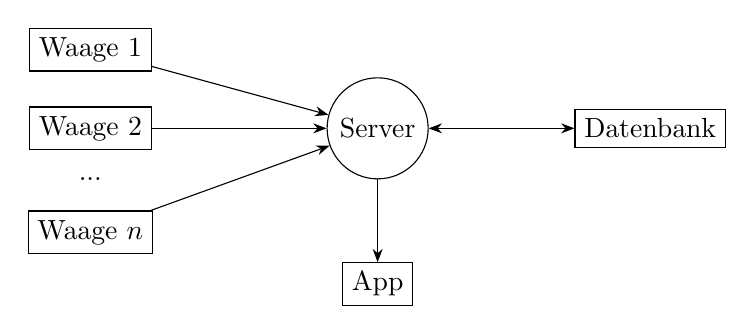
\begin{tikzpicture}

		\node[draw] (waage1) at (0,0) {Waage 1};
		\node[draw] (waage2) [below of = waage1] {Waage 2};
		\node[draw=none] (waage3) [below of = waage2, below = -0.5cm] {...};
		\node[draw] (waagen) [below of = waage3, below = -0.6cm] {Waage $n$};
		\node[draw, shape=circle] (server) [right of = waage2, right = 2cm] {Server};
		\node[draw] (app)    [below of = server, below = 0.7cm] {App};
		\node[draw] (data)   [right of = server, right = 1.5cm] {Datenbank};

		\draw[arrows=-Stealth] (waage1) -- (server);
		\draw[arrows=-Stealth] (waage2) -- (server);
		\draw[arrows=-Stealth] (waagen) -- (server);
		\draw[arrows=Stealth-Stealth] (server) -- (data);
		\draw[Stealth-] (app) -- (server);
	\end{tikzpicture}
	\caption{Netzwerk Diagramm\label{abb:networkdiagram}}
\end{figure}

Im Falle meiner Bienenstockwaage habe ich einen mir ein System überlegt in das man beliebig viele Waagen ein spannen kann.
Es besteht aus einem zentralen Server mit einer Datenbank kommunizieren kann.
Die einzelnen Bienenstockwaagen schicken ihre Daten an den zentralen Server welcher diese in Datenbank abspeichert.
Siehe Abbildung~\ref{abb:networkdiagram}.

Wenn man sich die Daten anschauen will, kann man dies über eine Webseite die mit Hilfe einer REST-API\footnote{Was eine REST-API ist können sie in Abschnitt~\ref{} lesen.} mit dem Server verbunden ist.

% Literaturverzeichnis {{{1
\printbibliography{}
\end{document}
